\documentclass[11pt]{article}

\usepackage{amsmath,amssymb,amsfonts}
\usepackage{dsfont}
\usepackage{listings}
\usepackage{xcolor}
\usepackage{graphicx}
\usepackage{bbm}
\usepackage{float}
%\usepackage{hyperref}
\usepackage{subfig}
\usepackage[breaklinks=true,colorlinks,citecolor=black,linkcolor=gfGG,urlcolor=gfFP]{hyperref}
% http://www.colourlovers.com/palette/92095/Giant_Goldfish
\definecolor{gfCD}{HTML}{69D2E7} % Cloudless Day
\definecolor{gfSP}{HTML}{A7DBD8} % Sunken Pool
\definecolor{gfBS}{HTML}{E0E4CC} % Beach Storm
\definecolor{gfGG}{HTML}{F38630} % Giant Goldfish
\definecolor{gfFP}{HTML}{FA6900} % Food Pills

\definecolor{codegreen}{rgb}{0,0.6,0}
\definecolor{codegray}{rgb}{0.5,0.5,0.5}
\definecolor{codepurple}{rgb}{0.58,0,0.82}
\definecolor{backcolour}{rgb}{0.95,0.95,0.92}
\lstdefinestyle{mystyle}{
    backgroundcolor=\color{backcolour},
    commentstyle=\color{codegreen},
    keywordstyle=\color{magenta},
    numberstyle=\tiny\color{codegray},
    stringstyle=\color{codepurple},
    basicstyle=\ttfamily\footnotesize,
    breakatwhitespace=false,
    breaklines=true,
    captionpos=b,
    keepspaces=true,
    numbers=left,
    numbersep=5pt,
    showspaces=false,
    showstringspaces=false,
    showtabs=false,
    tabsize=2
}

\setlength{\topmargin}{-.5in} \setlength{\textheight}{9.25in}
\setlength{\oddsidemargin}{0in} \setlength{\textwidth}{6.8in}

%\newcommand*{\SOLVE}{}%

\renewcommand{\vec}[1]{\mbox{\boldmath$#1$}}
\newcommand{\mm}[1]{\mathbf{#1}}

\newcounter{ProblemNum}
\newcounter{SubProblemNum}[ProblemNum]

\renewcommand{\theProblemNum}{\arabic{ProblemNum}}
\renewcommand{\theSubProblemNum}{\alph{SubProblemNum}}

\newcommand*{\anyproblem}[1]{\section*{#1}}
\newcommand*{\problem}[1]{\stepcounter{ProblemNum} %
   \anyproblem{Problem \theProblemNum \; (#1 points)}}
\newcommand*{\soln}[1]{\subsection*{#1}}
\newcommand*{\solution}{\soln{Solution}}
\newenvironment{solutions}
  {\section[Solution]{\textcolor{red}{Solution}}\color{red}}
  {\normalcolor}
\renewcommand*{\part}{\stepcounter{SubProblemNum} %
  \soln{Part (\theSubProblemNum)}}
\renewcommand{\theenumi}{(\alph{enumi})}
\renewcommand{\labelenumi}{\theenumi}
\renewcommand{\theenumii}{\roman{enumii}}
\let\endsection\relax
\let\endsubsection\relax

\graphicspath{
{.}
}
\lstset{style=mystyle}

\begin{document}

\Large
\noindent{\bf CS4851/6851 IDL: Homework 2 \hfill \today}
\medskip\hrule

\vspace{20pt}

Note: All coding problems to be submited with Github Link. Do not Upload the files/folder. Use git commands only.

Note: this is the distribution of questions:
\begin{enumerate}
  \item Question 1 to Question6: Required for everyone.
  \item Question 7: Required only for Graduate Students
\end{enumerate}



\problem{20} You have a convolutional neural network that takes as an
input image of size $512\times512\times3$ and passes it through a
layer that convolves the image using 3 filters of dimensions
$5\times5\times3$ with a valid padding.
\begin{enumerate}
 \item List all learnable parameters of this convolution layer.
 \item What if you want to replicate the behavior of this convolutional layer using a fully connected layer? How many parameters would that fully connected layer have?
\end{enumerate}


\problem{20} Given a binary input image of diagonal streaks (see
example in Figure~\ref{fig:image_example}) and two filters (see
Figure~\ref{fig:filters}) describe how would you build a detector for
finding the location of pattern shown in Figure~\ref{fig:Xpattern} on
the input image. Allowed operations are convolution, summation, and argmax.
\begin{figure}[ht]
  \centering
    \subfloat[Available fixed filters]{
    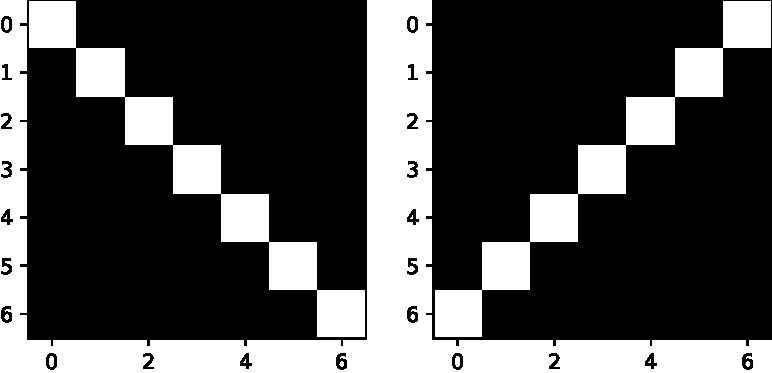
\includegraphics[height=4cm]{filters}
    \label{fig:filters}
  }
  \subfloat[Target shape to detect]{
    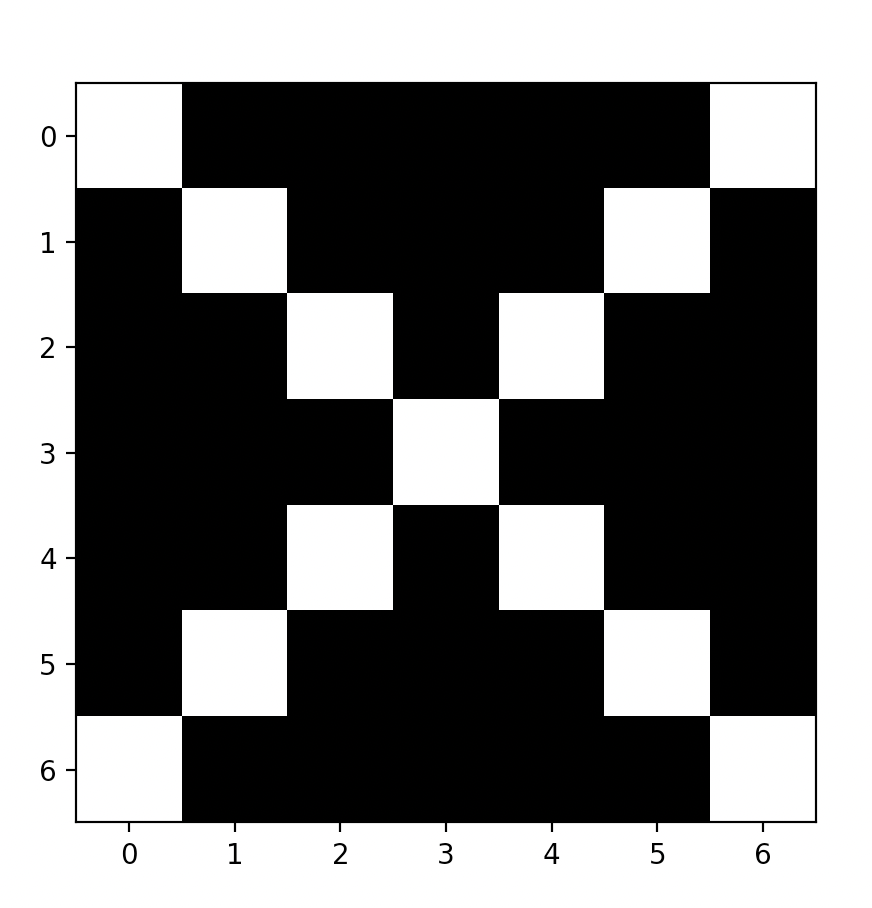
\includegraphics[height=4cm]{X}
    \label{fig:Xpattern}
  }
  \caption{Filters to use
    (\ref{fig:filters}) and pattern to find (\ref{fig:Xpattern}).}
        \label{fig:xfilters}
      \end{figure}
      
\begin{figure}[t]
  \begin{center}
    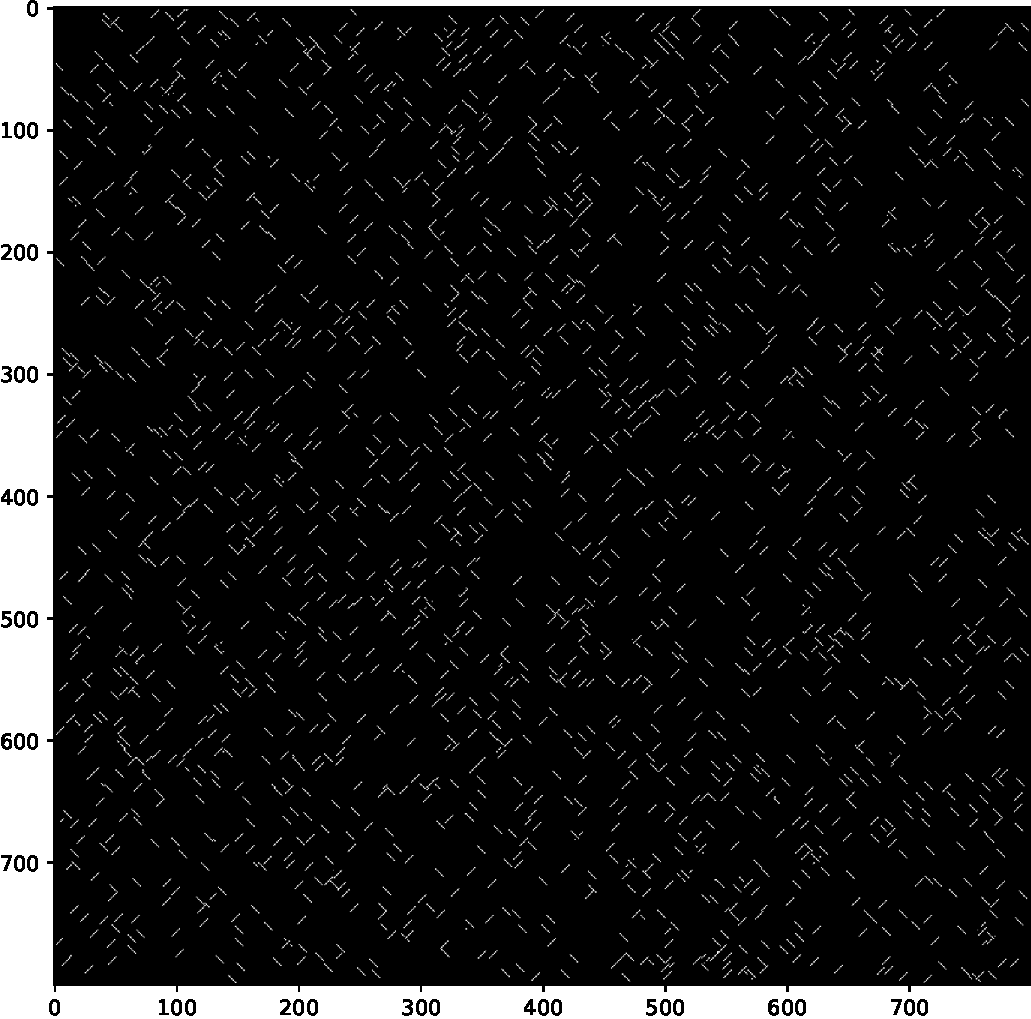
\includegraphics[width=1.0\textwidth]{pattern}
  \end{center}
  \caption{An example image for the architecture}
  \label{fig:image_example}
\end{figure}

\vspace{20pt}
\noindent\rule[0.5ex]{0.45\linewidth}{1pt} Bonus for undergraduates beyond this line

\problem{20}
Demonstrate that convolution is translation invariant for 1D convolution (Note:this can be extended to N-D convolutions as well).



\noindent\rule[0.5ex]{0.45\linewidth}{1pt} Bonus for both  undergraduates and graduates beyond this line.

\problem{20}
You have to choose between two papers given below: 
\begin{enumerate}
  \item Paper 1:
\href{https://arxiv.org/pdf/1102.0183.pdf}{High-Performance Neural
  Networks 
  for Visual Object Classification}:

\begin{enumerate}
\item Give a short summary of the paper.
\item What were the parameter sizes for CIFAR-10 and MNIST?  why do you think the paramtere size differed for CIFAR-10 vs MNIST?
\end{enumerate}

\item Paper 2:
\href{https://proceedings.neurips.cc/paper/2012/file/c399862d3b9d6b76c8436e924a68c45b-Paper.pdf}{ImageNet
  Classification with Deep Convolutional Neural Networks}:
\begin{enumerate}
\item Give a short summary of the paper.
\item Why is there a big fluctuation of loss for the last epoch of training?
\end{enumerate}
\end{enumerate}
% \vspace{2px}
\end{document}

%%% Local Variables:
%%% mode: latex
%%% TeX-master: t
%%% End:

